\chapter{RISC-V CPU}

This section provides a description of the CPU architecture and the functionality of its main modules.  
The RISC-V CPU design follows a classical five-stage organization:

\begin{itemize}
    \item Instruction Fetch (IF);
    \item Instruction Decode (ID);
    \item Execute (EX);
    \item Data Memory access (MEM);
    \item Write Back (WB).
\end{itemize}

It is important to note that the implemented design corresponds to a basic, non-pipelined architecture: each instruction traverses all stages sequentially, and the complete datapath is executed once per instruction.  
A more advanced implementation would include a pipelined architecture, which would require the introduction of pipeline registers between stages as well as the management of hazards (e.g., data hazards and control hazards).

This functionality has not been implemented in the current version; however, due to the modular structure of the project, the introduction of pipelining and hazard handling is feasible and can be considered as a possible future extension of the design.

The following sections provide a general overview of the role of the main components of the CPU. This document does not aim to cover the full set of technical details and specifications of the RISC-V architecture. For a complete and authoritative reference, the reader is referred to the official RISC-V documentation available on the \href{https://riscv.org/technical/specifications/}{RISC-V website}.

\pagebreak
\section{Instruction Fetch}

\begin{figure}[H]
  \centering
  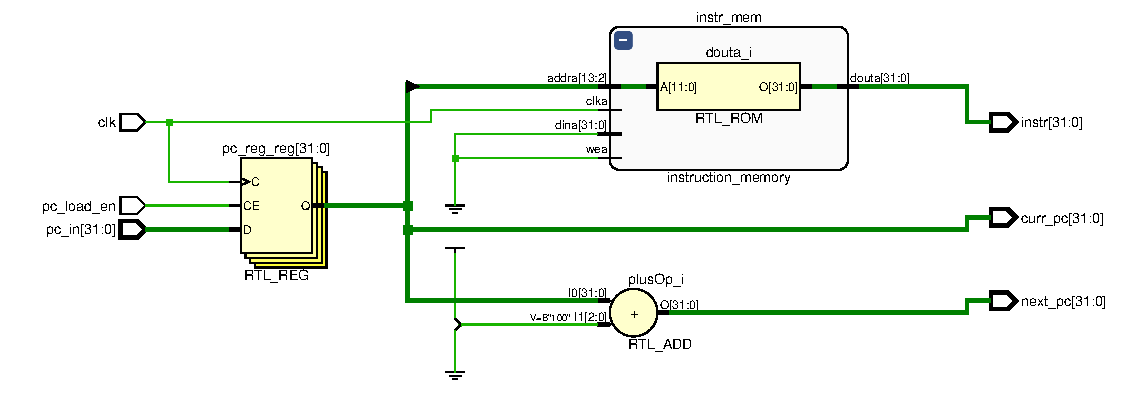
\includegraphics[width=\textwidth]{images/if_stage.pdf}
  \caption{High-level overview of the Instruction Fetch stage as rendered by Vivado.}
  \label{fig:if_stage}
\end{figure}

The Instruction Fetch (IF) stage manages the Program Counter, retrieves the current instruction from the instruction memory, and computes the address of the next sequential instruction. In the adopted single-cycle architecture, this stage enables a straightforward sequential execution model and provides the basis for future support of control-flow instructions such as branches and jumps.

The Program Counter is updated synchronously with the clock and only when the enable signal is asserted. The next instruction address is computed by adding four bytes to the current Program Counter value, while an externally provided target address can be loaded when required. The current Program Counter value and the fetched instruction are exposed to the subsequent stages of the processor.

For clarity, Listing~\ref{lst:if_entity} reports the interface of the Instruction Fetch stage, highlighting the main input and output signals.

{\scriptsize
\begin{lstlisting}[
    caption={Entity declaration of the Instruction Fetch stage.},
    label={lst:if_entity},
    breaklines=true,
    breakatwhitespace=true,
    columns=flexible
]
entity if_stage is
    port (
        clk         : in std_logic;
        pc_load_en  : in std_logic;                         -- enables PC loading
        pc_in       : in std_logic_vector(31 downto 0); -- value to load into PC

        next_pc     : out std_logic_vector(31 downto 0); -- PC + 4
        curr_pc     : out std_logic_vector(31 downto 0); -- current PC
        instr       : out std_logic_vector(31 downto 0)  -- fetched instruction
    );
end if_stage;
\end{lstlisting}
}

The Instruction Fetch stage has been validated using a dedicated testbench. During simulation, the fetched instructions are provided by the instruction memory module, which is initialized with a small test program. This allows the verification of the correct instruction fetch sequence and the sequential progression of the Program Counter.

The instruction memory used in the testbench contains the following test instructions, selected to exercise basic arithmetic and memory access operations.

{\scriptsize
\begin{lstlisting}[
    caption={Initialization of the instruction memory used for simulation.},
    label={lst:instr_mem_init},
    breaklines=true,
    breakatwhitespace=true,
    columns=flexible
]
signal rom : rom_t := (
    0 => x"00500093", -- addi x1, x0, 5
    1 => x"00A00113", -- addi x2, x0, 10
    2 => x"002081B3", -- add  x3, x1, x2
    3 => x"00302023", -- sw   x3, 0(x0)
    4 => x"00002203", -- lw   x4, 0(x0)
    others => (others => '0')
);
\end{lstlisting}
}

The testbench verifies the correct update of the Program Counter when enabled and the proper increment of the instruction address during sequential execution. The corresponding simulation results are reported in Figure~\ref{fig:tb_if_stage}.

\begin{figure}[H]
  \centering
  \includegraphics[width=\textwidth]{images/tb_if_stage.png}
  \caption{Simulation results of the Instruction Fetch testbench as rendered by Vivado.}
  \label{fig:tb_if_stage}
\end{figure}

\pagebreak
\section{Instruction Decode}

\begin{figure}[H]
  \centering
  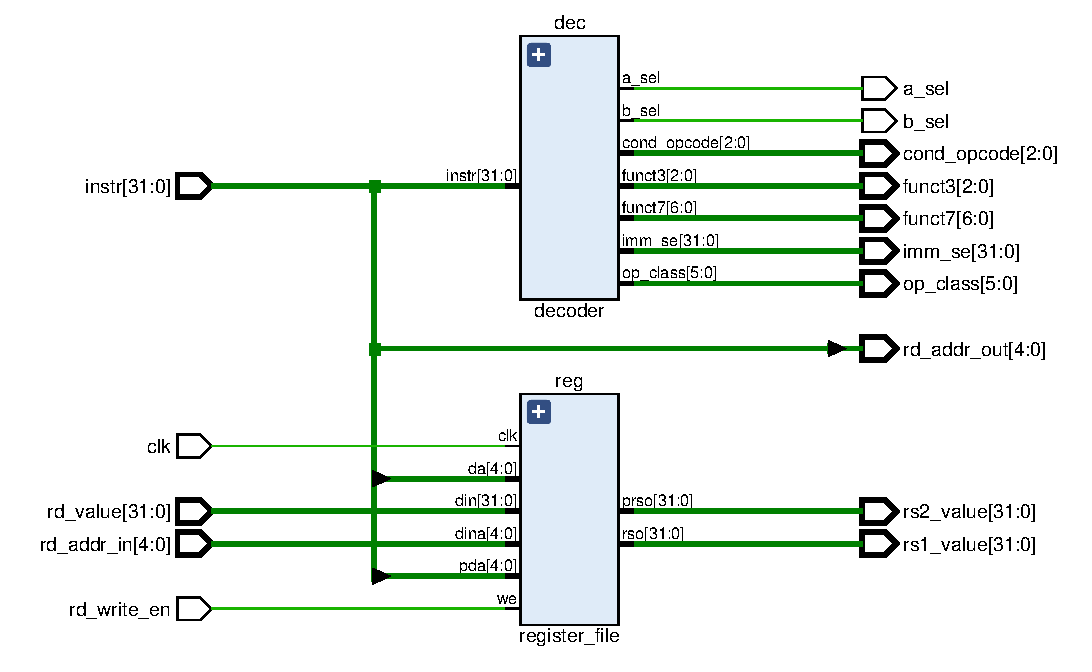
\includegraphics[width=\textwidth]{images/id_stage.pdf}
  \caption{High-level overview of the Instruction Decode stage as rendered by Vivado.}
  \label{fig:id_stage}
\end{figure}

The Instruction Decode (ID) stage is responsible for decoding the fetched instruction and for preparing all the information required by the subsequent execution stage. In particular, this stage extracts the opcode and function fields, selects the appropriate control signals, reads the source operands from the register file, and generates the sign-extended immediate value when required. The ID stage also handles the write-back interface, allowing register updates from the MEM/WB stage.

A high-level view of the Instruction Decode stage as synthesized and rendered by Vivado is shown in Figure~\ref{fig:id_stage}. The diagram highlights the main submodules involved in instruction decoding, register file access, and immediate generation.

The interface of the Instruction Decode stage is reported in Listing~\ref{lst:id_entity}. The entity exposes the fetched instruction as input, the write-back interface from the MEM/WB stage, and a set of decoded control signals and operands to be forwarded to the execution stage.

{\scriptsize
\begin{lstlisting}[
    caption={Entity declaration of the Instruction Decode stage.},
    label={lst:id_entity},
    breaklines=true,
    breakatwhitespace=true,
    columns=flexible
]
entity id_stage is
    port (
        clk         : in std_logic;
        instr       : in std_logic_vector(31 downto 0);

        -- Writeback interface (from MEM/WB stage)
        rd_write_en : in std_logic;
        rd_value    : in std_logic_vector(31 downto 0);
        rd_addr_in  : in std_logic_vector(4 downto 0);

        -- Decoded instruction information
        op_class    : out std_logic_vector(5 downto 0);
        funct3      : out std_logic_vector(2 downto 0);
        funct7      : out std_logic_vector(6 downto 0);
        a_sel       : out std_logic;
        b_sel       : out std_logic;
        cond_opcode : out std_logic_vector(2 downto 0);
        rd_addr_out : out std_logic_vector(4 downto 0);

        -- Operand values and immediate
        rs1_value   : out std_logic_vector(31 downto 0);
        rs2_value   : out std_logic_vector(31 downto 0);
        imm_se      : out std_logic_vector(31 downto 0)
    );
end id_stage;
\end{lstlisting}
}

The Instruction Decode stage has been verified through a dedicated testbench. The testbench initializes a register value through the write-back interface and then applies a sequence of instructions in order to validate correct operand reading, immediate generation, and instruction decoding. Listing~\ref{lst:id_tb_stim} reports an excerpt of the stimulus process used for verification.

{\scriptsize
\begin{lstlisting}[
    caption={Excerpt of the stimulus process used in the Instruction Decode testbench.},
    label={lst:id_tb_stim},
    breaklines=true,
    breakatwhitespace=true,
    columns=flexible
]
-- Stimulus
stim_proc : process
begin
    -- ===================================
    -- Write x1 = 0x00000010
    -- ===================================
    rd_write_en <= '1';
    rd_addr_in  <= "00001";
    rd_value    <= x"00000010";
    wait for clk_period;
    rd_write_en <= '0';

    -- ===================================
    -- ADDI x2, x1, 4
    -- ===================================
    instr <= x"00408113"; -- addi x2, x1, 4
    wait for clk_period;

    -- ===================================
    -- ADD x3, x1, x2
    -- ===================================
    instr <= x"002081B3"; -- add x3, x1, x2
    wait for clk_period;

    wait;
end process;
\end{lstlisting}
}

The simulation results obtained from the testbench are shown in Figure~\ref{fig:tb_id_stage}. The waveforms confirm the correct decoding of the instruction fields, the proper reading of the source registers, and the correct generation of the immediate values for immediate-type instructions.

\begin{figure}[H]
  \centering
  \includegraphics[width=\textwidth]{images/tb_id_stage.png}
  \caption{Simulation results of the Instruction Decode testbench as rendered by Vivado.}
  \label{fig:tb_id_stage}
\end{figure}

\pagebreak
\section{Instruction Execute}

\begin{figure}[H]
  \centering
  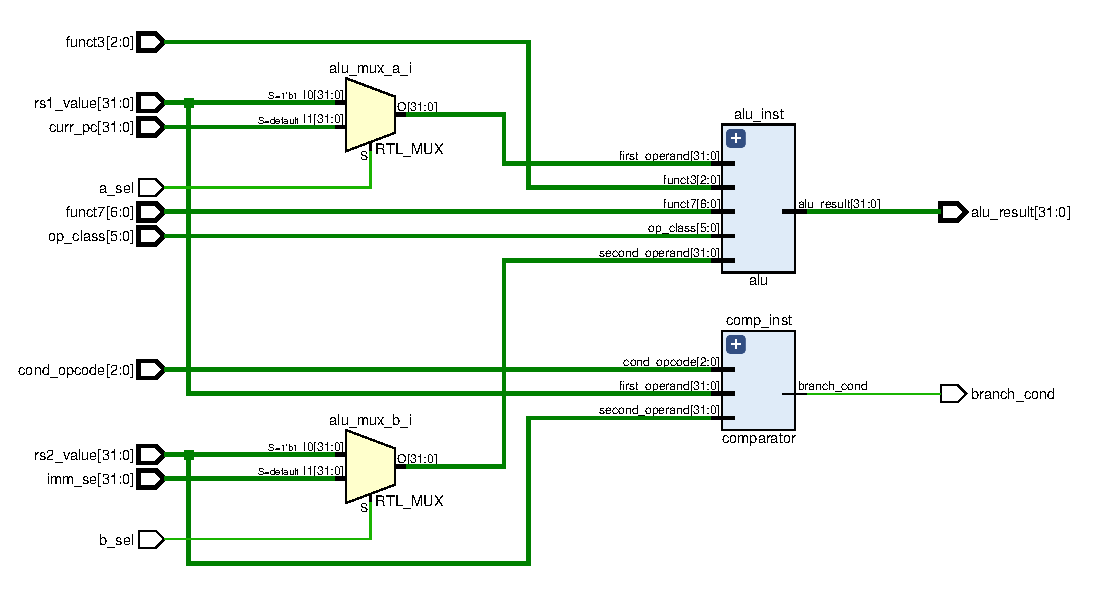
\includegraphics[width=\textwidth]{images/ex_stage.pdf}
  \caption{High-level overview of the Instruction Execute stage as rendered by Vivado.}
  \label{fig:ex_stage}
\end{figure}

The Instruction Execute (EX) stage is responsible for performing arithmetic and logical operations, computing branch conditions, and generating the intermediate results required by the subsequent stages of the datapath. This stage represents the computational core of the processor.

The EX stage includes two main functional units: an Arithmetic Logic Unit (ALU) and a comparator. The ALU performs arithmetic and logical operations such as addition, subtraction, and immediate-based computations. The comparator evaluates conditional expressions used by branch instructions, such as equality and signed or unsigned comparisons, and generates the corresponding branch condition signal. Based on the decoded instruction and control signals, the EX stage selects the appropriate operands and computes the final execution result.

A high-level view of the Instruction Execute stage as synthesized and rendered by Vivado is shown in Figure~\ref{fig:ex_stage}. The diagram highlights the integration of the ALU, the comparator, and the operand selection logic.

The interface of the Instruction Execute stage is reported in Listing~\ref{lst:ex_entity}. The entity exposes control signals for operand selection, the decoded instruction fields, and the data operands required by the ALU and comparator. The outputs include the computed ALU result and the evaluated branch condition.

{\scriptsize
\begin{lstlisting}[
    caption={Entity declaration of the Instruction Execute stage.},
    label={lst:ex_entity},
    breaklines=true,
    breakatwhitespace=true,
    columns=flexible
]
entity ex_stage is
    port (
        -- Control signals
        a_sel           : in std_logic;  -- 0 = PC,  1 = rs1
        b_sel           : in std_logic;  -- 0 = imm, 1 = rs2

        -- Data inputs
        rs1_value       : in std_logic_vector(31 downto 0);
        rs2_value       : in std_logic_vector(31 downto 0);
        imm_se          : in std_logic_vector(31 downto 0);
        curr_pc         : in std_logic_vector(31 downto 0);

        -- Decode information
        cond_opcode     : in std_logic_vector(2 downto 0);
        funct3          : in std_logic_vector(2 downto 0);
        funct7          : in std_logic_vector(6 downto 0);
        op_class        : in std_logic_vector(5 downto 0);

        -- Outputs
        branch_cond     : out std_logic;
        alu_result      : out std_logic_vector(31 downto 0)
    );
end ex_stage;
\end{lstlisting}
}

The Instruction Execute stage has been validated using a dedicated testbench that applies a set of representative instructions and input operands. The testbench verifies both arithmetic operations and branch condition evaluation, including register-based operations, immediate-based operations, and PC-relative computations. Listing~\ref{lst:ex_tb_stim} reports an excerpt of the stimulus process used for verification.

{\scriptsize
\begin{lstlisting}[
    caption={Excerpt of the stimulus process used in the Instruction Execute testbench.},
    label={lst:ex_tb_stim},
    breaklines=true,
    breakatwhitespace=true,
    columns=flexible
]
-- Stimulus process
stim_proc : process
begin
    -- =====================================
    -- ADD: x1 + x2
    -- =====================================
    rs1_value <= x"00000005";
    rs2_value <= x"00000003";
    a_sel     <= '1';
    b_sel     <= '1';
    op_class  <= "000001"; -- OP
    funct3    <= "000";
    funct7    <= "0000000";
    wait for 20 ns;

    -- =====================================
    -- SUB: x1 - x2
    -- =====================================
    funct7 <= "0100000";
    wait for 20 ns;

    -- =====================================
    -- ADDI: x1 + imm
    -- =====================================
    b_sel    <= '0';
    imm_se   <= x"00000004";
    op_class <= "000010"; -- OP-IMM
    funct7   <= "0000000";
    wait for 20 ns;

    -- =====================================
    -- AUIPC: PC + imm
    -- =====================================
    a_sel    <= '0';
    curr_pc  <= x"00001000";
    imm_se   <= x"00000010";
    op_class <= "010010";
    wait for 20 ns;

    -- =====================================
    -- BEQ (true)
    -- =====================================
    rs1_value   <= x"0000000A";
    rs2_value   <= x"0000000A";
    cond_opcode <= "000"; -- BEQ
    op_class    <= "100000"; -- BRANCH
    wait for 20 ns;

    -- =====================================
    -- BLT (signed, false)
    -- =====================================
    rs1_value   <= x"00000005";
    rs2_value   <= x"00000002";
    cond_opcode <= "100"; -- BLT
    wait for 20 ns;

    wait;
end process;
\end{lstlisting}
}

The simulation results obtained from the testbench are shown in Figure~\ref{fig:tb_ex_stage}. The waveforms confirm the correct computation of ALU results and the correct evaluation of branch conditions for the tested instruction set.

\begin{figure}[H]
  \centering
  \includegraphics[width=\textwidth]{images/tb_ex_stage.png}
  \caption{Simulation results of the Instruction Execute testbench as rendered by Vivado.}
  \label{fig:tb_ex_stage}
\end{figure}

\pagebreak
\section{Data Memory}

\begin{figure}[H]
  \centering
  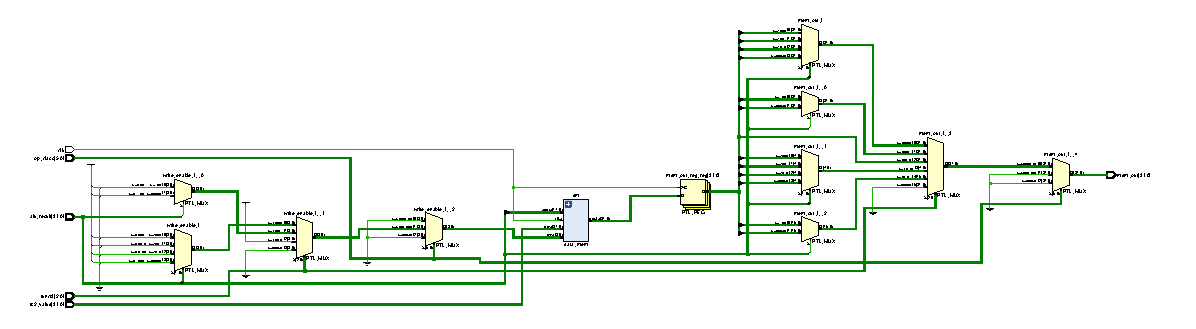
\includegraphics[width=\textwidth]{images/mem_stage.pdf}
  \caption{High-level overview of the Data Memory stage as rendered by Vivado.}
  \label{fig:mem_stage}
\end{figure}

The Data Memory (MEM) stage is responsible for handling memory access operations generated by load and store instructions. In this stage, the address computed by the execution stage is used to access the data memory, either to read a value from memory (load operations) or to write a value to memory (store operations). This stage therefore provides the interface between the CPU core and the data memory subsystem. The write-back of loaded values to the register file is handled in the subsequent stage.

In the current design, the Data Memory stage instantiates a dedicated memory module, referred to as data\_mem, which implements the actual storage element. The MEM stage is responsible for decoding the operation type and for driving the appropriate control signals to the memory module.

A high-level view of the Data Memory stage as synthesized and rendered by Vivado is shown in Figure~\ref{fig:mem_stage}.

The interface of the Data Memory stage is reported in Listing~\ref{lst:mem_stage_entity}. The entity receives the operation class and function fields required to identify the memory operation, the data to be written in case of store instructions, and the address computed by the execution stage. The output provides the value read from memory in case of load instructions.

{\scriptsize
\begin{lstlisting}[
    caption={Entity declaration of the Data Memory stage.},
    label={lst:mem_stage_entity},
    breaklines=true,
    breakatwhitespace=true,
    columns=flexible
]
entity mem_stage is
    port ( 
        clk         : in std_logic;
        op_class    : in std_logic_vector(5 downto 0);
        funct3      : in std_logic_vector(2 downto 0);
        rs2_value   : in std_logic_vector(31 downto 0);
        alu_result  : in std_logic_vector(31 downto 0);

        mem_out     : out std_logic_vector(31 downto 0)
    );
end mem_stage;
\end{lstlisting}
}

The actual memory storage is implemented by the data\_mem module, whose interface is reported in Listing~\ref{lst:data_mem_entity}. This module provides a simple synchronous write and asynchronous read interface and is accessed using the address generated by the execution stage.

{\scriptsize
\begin{lstlisting}[
    caption={Entity declaration of the data memory module.},
    label={lst:data_mem_entity},
    breaklines=true,
    breakatwhitespace=true,
    columns=flexible
]
entity data_mem is
    port(
        clka  : in std_logic;
        wea   : in std_logic_vector(3 downto 0);
        dina  : in std_logic_vector(31 downto 0);
        addra : in std_logic_vector(11 downto 0);

        douta : out std_logic_vector(31 downto 0)
    );
end data_mem;
\end{lstlisting}
}

\pagebreak
\section{Write Back}

\begin{figure}[H]
  \centering
  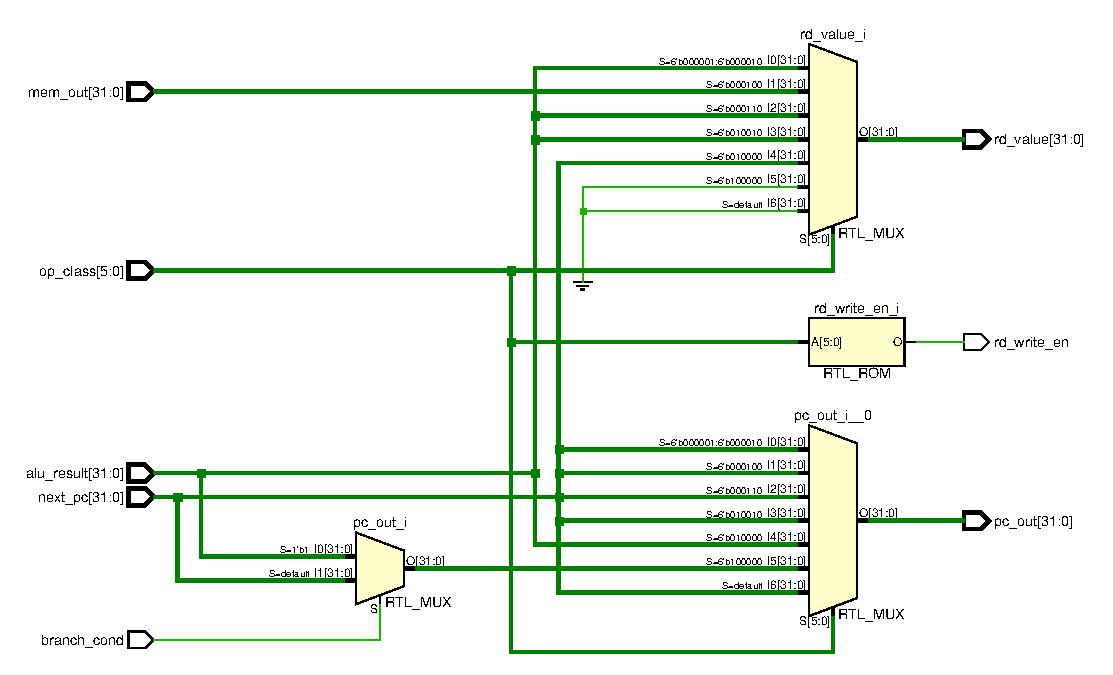
\includegraphics[width=\textwidth]{images/wb_stage.pdf}
  \caption{High-level overview of the Write Back stage as rendered by Vivado.}
  \label{fig:wb_stage}
\end{figure}

The Write Back (WB) stage is responsible for completing the execution of an instruction by writing the final result back to the register file and by updating the Program Counter when required. This stage selects the correct result source depending on the instruction type, such as the ALU output for arithmetic and logical operations or the memory output for load instructions. In addition, the WB stage handles control-flow updates by providing the next Program Counter value in case of branch instructions.

A high-level view of the Write Back stage as synthesized and rendered by Vivado is shown in Figure~\ref{fig:wb_stage}. The diagram highlights the selection logic used to route the correct result to the register file and to determine the next value of the Program Counter.

The interface of the Write Back stage is reported in Listing~\ref{lst:wb_entity}. The entity receives the execution results and control information from the previous stages and produces the control signals required to update the register file and the Program Counter.

{\scriptsize
\begin{lstlisting}[
    caption={Entity declaration of the Write Back stage.},
    label={lst:wb_entity},
    breaklines=true,
    breakatwhitespace=true,
    columns=flexible
]
entity wb_stage is
    port ( 
        branch_cond : in std_logic;
        op_class    : in std_logic_vector(5 downto 0);
        mem_out     : in std_logic_vector(31 downto 0);
        next_pc     : in std_logic_vector(31 downto 0);
        alu_result  : in std_logic_vector(31 downto 0);

        rd_write_en : out std_logic;
        pc_out      : out std_logic_vector(31 downto 0);
        rd_value    : out std_logic_vector(31 downto 0)
    );
end wb_stage;
\end{lstlisting}
}

The combined behavior of the Data Memory and Write Back stages has been verified through a dedicated testbench. The testbench applies a sequence of store and load instructions in order to validate correct memory accesses and proper forwarding of the loaded values to the write-back stage. Listing~\ref{lst:wb_tb_stim} reports an excerpt of the stimulus process used for verification.

{\scriptsize
\begin{lstlisting}[
    caption={Excerpt of the stimulus process used in the MEM/WB testbench.},
    label={lst:wb_tb_stim},
    breaklines=true,
    breakatwhitespace=true,
    columns=flexible
]
-- Stimulus
stim_proc : process
begin
    -- =================================
    -- SW: store word
    -- =================================
    op_class   <= "001000"; -- STORE
    funct3     <= "010";    -- SW
    alu_result <= x"00000000";
    rs2_value  <= x"DEADBEEF";
    wait for clk_period;

    -- =================================
    -- LW: load word
    -- =================================
    op_class   <= "000100"; -- LOAD
    funct3     <= "010";    -- LW
    alu_result <= x"00000000";
    wait for clk_period;

    -- =================================
    -- LB (signed)
    -- =================================
    funct3     <= "000";
    alu_result <= x"00000000";
    wait for clk_period;

    -- =================================
    -- LBU (unsigned)
    -- =================================
    funct3     <= "100";
    wait for clk_period;

    wait;
end process;
\end{lstlisting}
}

The simulation results obtained from the MEM/WB testbench are shown in Figure~\ref{fig:tb_wb_stage}. The waveforms confirm the correct handling of store and load operations, as well as the proper forwarding of memory data to the write-back stage.

\begin{figure}[H]
  \centering
  \includegraphics[width=\textwidth]{images/tb_mem_wb_stage.png}
  \caption{Simulation results of the Data Memory and Write Back testbench as rendered by Vivado.}
  \label{fig:tb_wb_stage}
\end{figure}

\pagebreak
\section{Datapath}

This section describes the datapath module, which represents the top-level integration of the CPU core. The datapath is implemented as a dedicated VHDL file whose purpose is to interconnect all the previously described stages, namely Instruction Fetch, Instruction Decode, Execute, Data Memory, and Write Back.

The datapath module defines the complete flow of data and control signals across the processor, connecting the output of each stage to the input of the subsequent one. In this way, it establishes the full execution path from instruction fetch to write back, enabling the coordinated operation of all stages within the single-cycle CPU architecture.

The datapath has been verified using a dedicated testbench that executes a small test program stored in the instruction memory. The sequence of instructions used during simulation is written in Listing~\ref{lst:instr_mem_init}.

These instructions allow the validation of immediate operations, register-to-register arithmetic, memory store operations, and memory load operations within the complete datapath.

The simulation results of the datapath testbench are shown in Figure~\ref{fig:tb_cpu_top}.

\begin{figure}[H]
  \centering
  \includegraphics[width=\textwidth]{images/tb_cpu_top.png}
  \caption{Simulation results of the datapath testbench as rendered by Vivado.}
  \label{fig:tb_cpu_top}
\end{figure}

During simulation, the values observed at the output of the ALU and at the Write Back stage are reported below:

\begin{center}
\begin{tabular}{c c l}
\hline
Value & Decimal & Source \\
\hline
5     & 5       & addi x1, x0, 5 \\
A     & 10      & addi x2, x0, 10 \\
F     & 15      & add x3, x1, x2 = 5 + 10 \\
0     & 0       & address computation for sw and lw (x0 + 0) \\
\hline
\end{tabular}
\end{center}

The ALU and Write Back output signals exhibit the same values during execution because the implemented architecture follows a single-cycle model. In each clock cycle, the result produced by the ALU is immediately propagated to the Write Back stage without intermediate pipeline registers. As a consequence, the values observed at the ALU output and at the Write Back interface coincide for the executed instructions.

The observed values (5, 10, 15, and 0) correspond respectively to the two immediate additions, the register-to-register addition, and the address computation used by the store and load instructions. This behavior confirms the correct propagation of data through the datapath and validates the functional correctness of the integrated CPU architecture.
